\documentclass{article}
\textheight		= 21cm
\textwidth		= 18cm
\topmargin		= -1cm
\oddsidemargin	= -1cm

\usepackage[spanish]{babel}
\usepackage[utf8]{inputenc}%%%Paquete para la acentuación, no hace falta poner \'vocal.
\usepackage{graphicx}
\usepackage{color}
\usepackage{hyperref}
\usepackage{enumitem}
\usepackage{subfig}
\usepackage{epsfig}
\usepackage{import}

\renewcommand{\labelitemi}{$\bullet$}

\graphicspath{{resources/}}
	
\hypersetup{%
  colorlinks=true,%
  linkcolor=blue,%
  citecolor=blue,%
  unicode,%
  pdfborder={0 0 0}%
}

\makeatletter
\newcommand{\logo}[2] {%
	\def\input@path{{#1}}
	\def\logoimg{#2}
}
\newcommand\version[1]{\renewcommand\@version{#1}}
\newcommand\@version{\@latex@error{No \noexpand\version given}\@ehc}
\makeatother

\begin{document}

\logo{resources}{ZambaLogo1-4a}
\version{ @LATEX_VERSION@ }
\title{Guía rápida del usuario}
\import{@CONFIG_PATH@/doxygen/}{title.tex}

\tableofcontents

\section{Introducción}

\textit{ZaMBA} es un software diseñado para funcionar como interfaz de control de los decodificadores del Sistema Argentino de Televisión Digital, con integración del middleware \textit{Ginga}, específicamente la implementación de \textit{Ginga.ar}.

Este software integra una interfaz de usuario simplificada y optimizada gráficamente, que permite la administración de canales (scanneo, listado de canales, bloqueo de no deseados, selección de favoritos), control parental, control de volumen, cambio de canal, configuración de video y audio, soporte para Guía Electrónica de Canales (EPG) y la vista rápida de información de programas, entre otras funciones.

\vspace{0.5cm}
\begin{figure}[h]
 \centerline{
\includegraphics[scale=0.8,keepaspectratio=true]{zamba}}
 \caption{ZaMBA - Lifia - U.N.L.P.}
\end{figure}
\pagebreak

\section{Comienzo}

Al iniciar el Set Top Box por primera vez, con el \textit{ZaMBA} instalado, se puede visualizar el Menú principal con el foco sobre la solapa \textbf{Canales} para poder realizar la búsqueda de los mismos.

En la siguiente figura \textbf{no} se visualiza el video principal, porque se debe realizar la búsqueda de canales.

\vspace{0.5cm}
\begin{figure}[h]
 \centerline{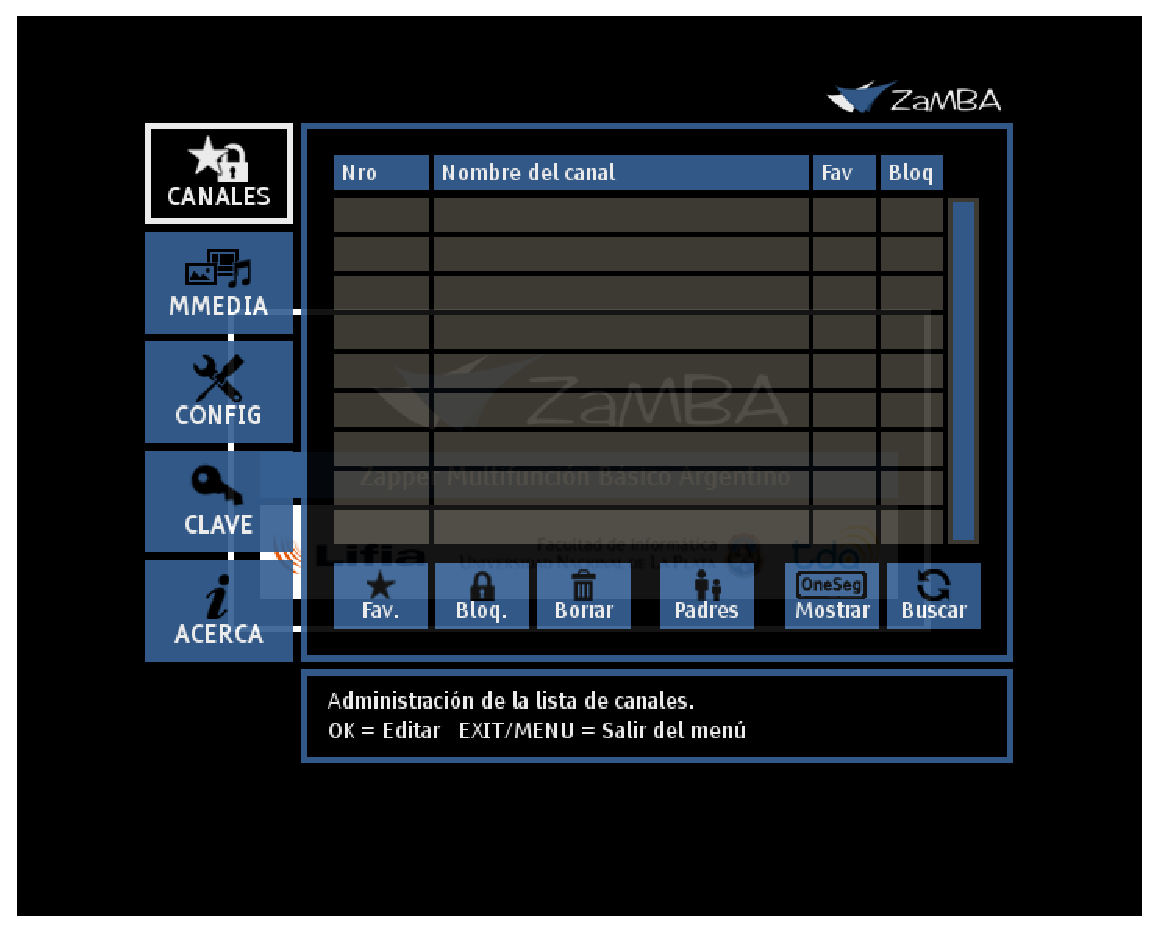
\includegraphics[scale=0.50,keepaspectratio=true]{inicio}}
 \caption{Vista inicial del Zapper}
\end{figure}
\pagebreak

% Funcionalidades
\section{Funcionalidad del Zapper}

\subsection{Info}
Se dispone de dos niveles de visualización de la información. 
En el primer nivel se muestra:
	\begin{itemize}
		\item Fecha.
		\item Hora.
		\item Nombre del canal.
		\item Resolución del video y tipo de audio.
		\item El tipo de contenido del programa actual.
		\item Nombre del programa que actualmente se esta transmitiendo junto con toda la información de este.
	\end{itemize}
	
	\begin{figure}[h]
 		\centerline{\includegraphics[scale=0.5,keepaspectratio=true]{info1}}
		\caption{Primer nivel de info}
	\end{figure}
	
En el segundo nivel se agrega al anterior la calidad e intensidad de la señal, junto con los servicios extra que pueda tener.
Estos pueden ser: múltiples audios o videos, Closed Caption y aplicaciones interactivas.

\subsection{EPG}
La guía electrónica de programas (siglas en inglés de \textbf{E}lectronic \textbf{P}rogram \textbf{G}uide) es donde se encuentran organizados de manera rápida y sencilla, todos los canales que nos ofrece un distribuidor de televisión. Así el usuario puede hacer una elección de lo que desea ver por televisión, sin necesidad de recurrir al habitual zapping.

\subsection{Lista de canales}
	\begin{enumerate}[label*=\arabic*.]
	\item 
\includegraphics[scale=0.60,keepaspectratio=true]{buscar} Realiza un scanneo completo de todas las frecuencias y almacena los canales disponibles.
	Si se encuentra definida una clave, se solicitará el ingreso de la misma, antes de realizar una nueva búsqueda de canales.
	\item 
\includegraphics[scale=0.60,keepaspectratio=true]{mostrar} Muestra u oculta los servicios OneSeg.
	\item 
\includegraphics[scale=0.60,keepaspectratio=true]{fav} Indica mostrando una \textit{estrella}, un canal como \textit{Favorito}. Posteriormente a esta operación, se podrán navegar los servicios señalizados, con el botón específico del control remoto.
	\item 
\includegraphics[scale=0.60,keepaspectratio=true]{bloq} Bloquea un canal determinado, mostrándolo con un ``candado'' en la lista de servicios disponibles. Si se requiere sintonizar el canal bloqueado, hay que hacerlo indicando el número de canal virtual y al sintonizar este servicio, se solicitará la clave de desbloqueo.
	\item 
\includegraphics[scale=0.60,keepaspectratio=true]{borrar} Borra un canal determinado, de la lista de canales disponible. 
	Si se desea recuperar el servicio borrado, hay que sintonizar todos los canales nuevamente, desde el menú \textit{Buscar}
	\end{enumerate}

\begin{figure}[h]
 \centerline{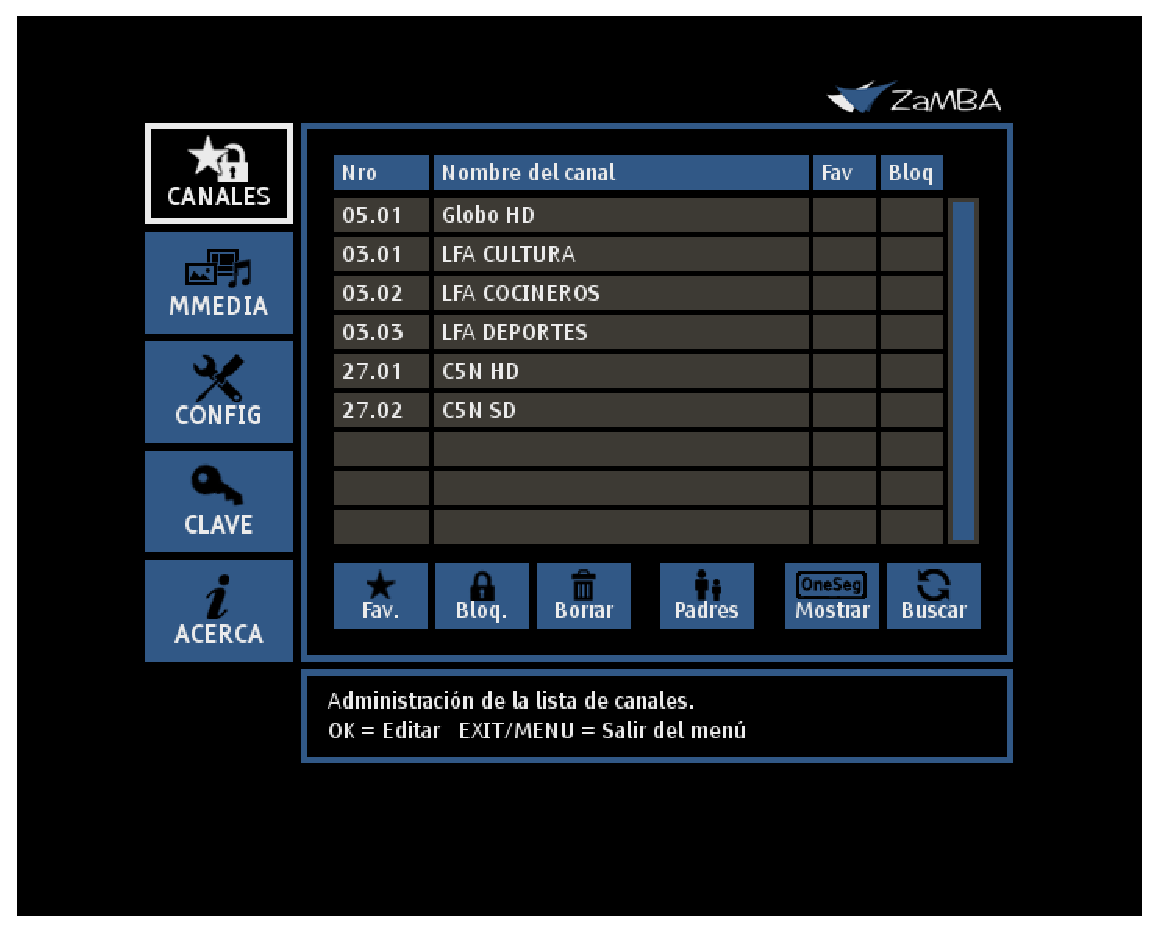
\includegraphics[scale=0.50,keepaspectratio=true]{canales}}
 \caption{Administración de los canales.}
\end{figure}
\pagebreak


\subsection{Contenidos} 
	\begin{enumerate}[label*=\arabic*.]
	\item 
\includegraphics[scale=0.60,keepaspectratio=true]{apps} Muestra la lista de aplicaciones disponibles. Éstas son las aplicaciones \textit{ZaMBA} habilitadas, más las aplicaciones \textit{Ginga} que se encuentran en el servicio sintonizado y/o almacenadas en un dispositivo USB.
	\item 
\includegraphics[scale=0.60,keepaspectratio=true]{images} Muestra las imágenes disponibles que se encuentran en un dispositivo USB.
	\item 
\includegraphics[scale=0.60,keepaspectratio=true]{music} Muestra la música disponible que se encuentra en un dispositivo USB.
	
Los formatos soportados son: MP3, ...
	\item \includegraphics[scale=0.60,keepaspectratio=true]{videos} Muestra los videos disponibles que se encuentran en un dispositivo USB.
		
Los formatos soportados son: MP4, ...
	\end{enumerate}

\begin{figure}[h]
 \centerline{\includegraphics[scale=0.50,keepaspectratio=true]{contenidos}}
 \caption{Listado de aplicaciones interactivas, música e imágenes.}
\end{figure}
\pagebreak

\subsection{Ajustes}

\begin{figure}[h]
 \centerline{\includegraphics[scale=0.50,keepaspectratio=true]{ajustes}}
 \caption{Ajustes del Set Top Box.}
\end{figure}

\subsubsection{Audio/Video}
	\begin{enumerate}[label*=\arabic*.]
	\item \textbf{Salida de video}, permite la configuración de los siguientes formatos soportados provistos en el \textit{Set Top Box:} Video Compuesto, por Componentes y HDMI.
	\item \textbf{Resolución}, las opciones de esta configuración se encuentra directamente relacionada con la configuración de \textit{Salida de Video}
	\item \textbf{Audio}, se puede definir como: Mono o Estéreo.
	\item \textbf{Opacidad del Menú}, permite configurar la opacidad con la que se visualizan los menues. 
	
El valor mínimo es \textbf{1 (uno)}, que muestra el menú transparente y el valor máximo es \textbf{10 (diez)}, y el menú no muestra transparencia.
	\end{enumerate}
	
	\begin{figure}[h]
		\centerline{\includegraphics[scale=0.50,keepaspectratio=true]{ajustes_av}}
		\caption{Ajustes de Audio/Video.}
	\end{figure}
	
\subsubsection{Aplicaciones}
	Las aplicaciones son software que extienden la funcionalidad de \emph{ZaMBA}; pueden ser de dos tipos, interactivas o servicios.\\
Las aplicaciones interactivas son aplicaciones que interactúan directamente con el usuario. Un juego es un ejemplo típico de aplicación interactiva. Para que puedan ser ejecutadas desde el listado de aplicaciones, es necesario que sean habilitadas.\\
Las aplicaciones de tipo servicio son aplicaciones que no interactúan directamente con el usuario. Un ejemplo típico es un servicio que mantiene e informa estadísticas sobre los canales que son vistos por el usuario. Para activar un servicio sólo es necesario habilitarlo.\\
Dentro de cada aplicación hay un botón \texttt{configuración} el cual estará disponible siempre que una aplicación esté habilitada y sea configurable, éste botón permite desplegar el menú de configuración; las opciones a configurar dependen de cada aplicación en particular.\\

	\begin{figure}[h]
		\centerline{\includegraphics[scale=0.50,keepaspectratio=true]{ajustes_apps}}
		\caption{Ajustes de aplicaciones.}
	\end{figure}
	
\subsubsection{Red}
	Permite visualizar las interfaces de red presentes, pudiendo seleccionar una y ver su configuración actual.
	
	\begin{figure}[h]
		\centerline{\includegraphics[scale=0.50,keepaspectratio=true]{ajustes_red}}
		\caption{Ajustes de red.}
	\end{figure}

\subsubsection{Seguridad}
	Permite definir, modificar o eliminar una clave numérica de cuatro dígitos, que servirá para la autenticación de las funciones de restricción de contenido, como el bloqueo de canales y el control parental.
	La primera vez que se ingresa se solicitará que establezca la clave y luego se habilitarán el resto de las opciones:
	
	\begin{enumerate}[label*=\arabic*.]
	\item \textbf{Modificar clave}, permite cambiar la clave actual por una nueva.
	\item \textbf{Eliminar clave}, elimina la clave actual. Por consiguiente se deshabilitarán todas las opciones relacionadas con restricción de contenido.
	\item \textbf{Duración de sesión}, permite seleccionar el tiempo por el cual la sesión permanecerá abierta desde la última autenticación.
	\item \textbf{Cerrar sesión}, cierra la sesión actual. Cualquier acción próxima relacionada con restricción de contenido requerirá que se vuelva a ingresar la clave.
	\item \textbf{Cerrar sesión}, cierra la sesión actual. Cualquier acción próxima relacionada con restricción de contenido.
	\item \textbf{Control Parental}, permite restringir el acceso al contenido televisivo mediante el control parental, definiendo una clave previamente.
	
Esta función dispone de dos tipos de filtrado:
	\begin{itemize}
	\item \textbf{Por edad:} Existe la posibilidad de elegir el filtrado para mayores de 10, 12, 14, 16 y 18 años.
	\item \textbf{Por contenido:} Permite el filtrado por Violencia, Sexo o Drogas.
	\end{itemize}
	
	\end{enumerate}
	
	\begin{figure}[h]
		\centerline{\includegraphics[scale=0.50,keepaspectratio=true]{ajustes_seguridad}}
		\caption{Ajustes de seguridad.}
	\end{figure}

\subsubsection{Actualización}
	En esta sección se puede configurar la forma en que se actualizará el sistema. Se cuenta con dos formas:
	\begin{itemize}
		\item \textbf{Actualización OTA} Estas actualizaciones llegarán por el aire, es decir por el mismo medio que llega la señal de televisión.
		\item \textbf{Actualización por red} Estas actualizaciones llegarán por medio de la red que tenga configurada el Set Top Box, puede ser cableada o por Wi-Fi.
	\end{itemize}
	
	\begin{figure}[h]
		\centerline{\includegraphics[scale=0.50,keepaspectratio=true]{ajustes_actualizacion}}
 		\caption{Configuración de actualizaciones.}
	\end{figure}

\subsubsection{Restaurar}
	Aquí se podrán restaurar los valores de fabrica. Todos los cambios hechos en ajustes serán perdidos.
	
	\begin{figure}[h]
		\centerline{\includegraphics[scale=0.50,keepaspectratio=true]{ajustes_restaurar}}
 		\caption{Restaurar ajustes.}
	\end{figure}
	
\pagebreak

\subsection{Acerca} Muestra la versión actual del Zapper y brinda una breve reseña de su funcionamiento.

\begin{figure}[h]
 \centerline{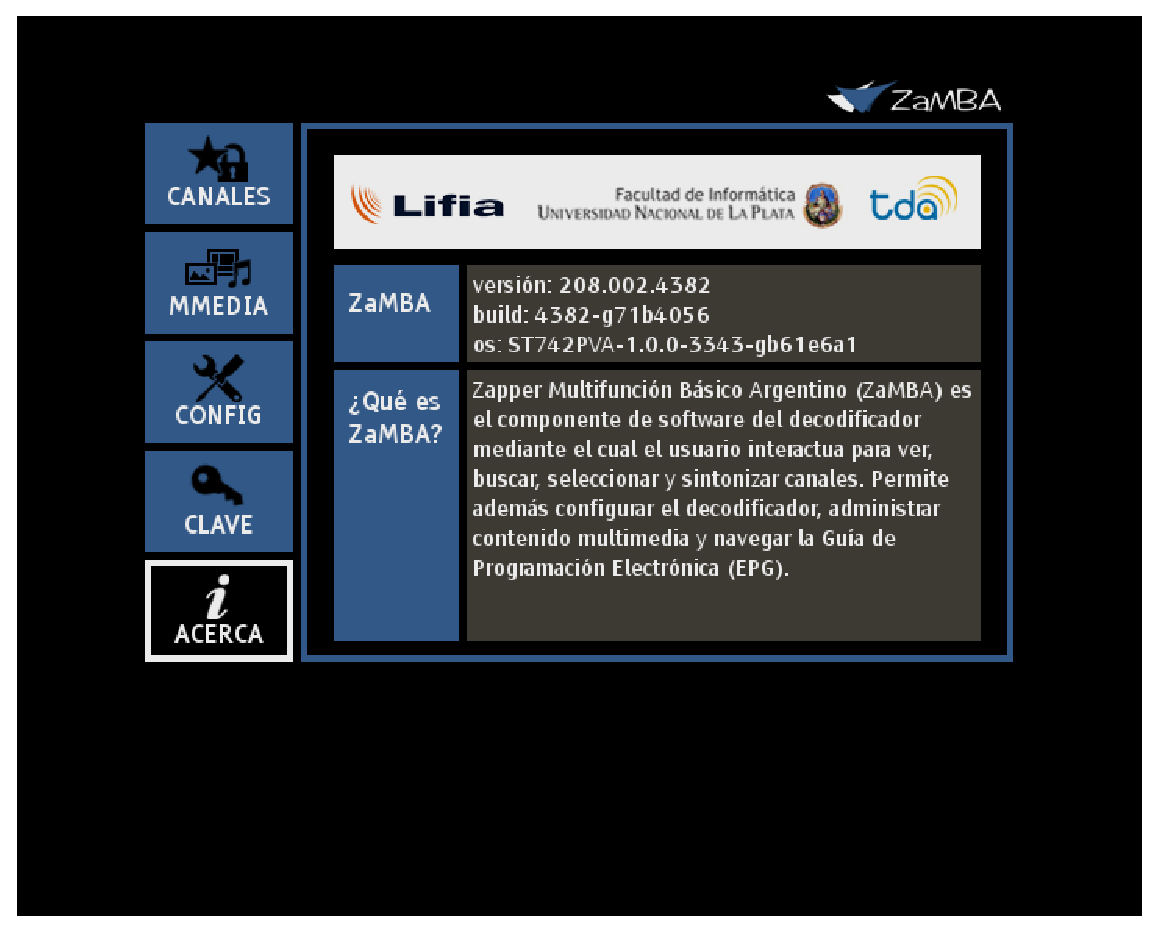
\includegraphics[scale=0.50,keepaspectratio=true]{acerca}}
 \caption{Información y Versión de Zapper.}
\end{figure}

\end{document}